The success of transfer learning suggests that exploiting the knowledge of the existing models properly can greatly help us to learn new data. 
Transfer learning on image recognition is a very popular topic in recent years. Domain adaptation for image recognition tries to exploit the knowledge from a source domain with a plentiful data to help learn a classifier for the target domain with a different distribution and little labeled training data. In domain adaptation, the source and target domains share the same label but their data are drawn from the different distribution.

In domain adaptation, the knowledge of the source domain can be transferred in 3 different approaches: instance , model and feature representation transfer \cite{pan2010survey}. In this paper, we propose a method that transfers the knowledge from the source model. Some recent works show that exploiting the knowledge from the source model can boost the performance of the target model effectively. Tommasi et al. \cite{tommasi2014learning} show that it is possible to learn a good target model with just a few positive examples. Kuzborskij et al.\cite{kuzborskij2013n} show that leveraging the knowledge from the source models is more effective than the source data.
Moreover, in some real applications, we can only obtain the source models and it is difficult to access their training data because of various of reasons such as the data credential.   
Recently, a framework called Hypothesis Transfer Learning (HTL) has been proposed to handle this situation \cite{kuzborskij2013stability}. HTL assumes only source models (called the \textit{hypotheses}) trained on source task can be utilized and there is no access to source data, nor any knowledge about the relatedness of the source and target distributions. 
In HTL, a number of works have been attempted with Least Square Support Vector Machine (LS-SVM) as LS-SVM is widely used in pattern recognition \cite{bishop2006pattern}. Previous approaches show that the hypotheses can be evaluated effectively with LS-SVM via Leave-One-Out cross-validation \cite{tommasi2014learning}.

\begin{figure}[h]
\centering
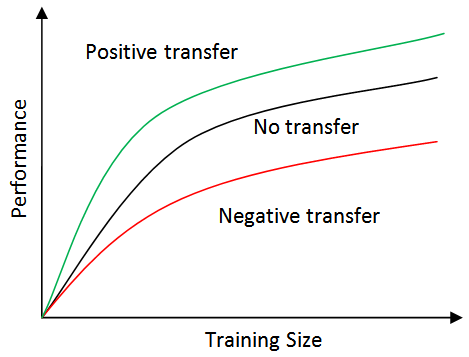
\includegraphics[scale=.4]{fig/negative.png}
\caption{Relying on the related source knowledge can improve the performance of the target model while forcing the target model to rely on the unrelated source could suffer from negative transfer.}
\end{figure}

In domain adaptation, different source domain can make the different contribution to the performance of the target model.
The theoretical research shows that the utility of the source domain decreases as the distributions of the source and target data become less similar (or \textit{less related})  \cite{ben2010theory} \cite{ben2007analysis}. Moreover, when the source and target tasks are not related, negative transfer may happen. In transfer learning, \textit{negative transfer} 
refers to the phenomenon where the source knowledge hurts the learning process and degrades the performance of the target model compare to a method without using any source knowledge \cite{pan2010survey}. 
Previous work of HTL assumes that the source and target domains are still very related. Most of them just consider the scenario where the target task is adding a new category to the source task (so called \textit{from N classes to N+1 classes}) \cite{tommasi2014learning} \cite{kuzborskij2013n} \cite{jie2011multiclass}. Moreover, their algorithms only focus on the performance on the newly added category, i.e. binary classification scenario, while paying less attention to the performance of the target model on all classes in the target data (the multi-class scenario). In domain adaptation, the source and target domains can be related in different level (from strongly related to weakly related), negative transfer could happen when they are weakly related. This could be a more severe issue when we consider the performance of the target model on the whole target data (see Figure \ref{fig:distribution}).

%Previous works \cite{tommasi2014learning}, \cite{kuzborskij2013n} suggest that to better utilizing the hypotheses and reduce negative transfer, the decision of the algorithm should be made by combining the prior hypotheses and empirical knowledge (from the specific target task).

\begin{figure}
\centering
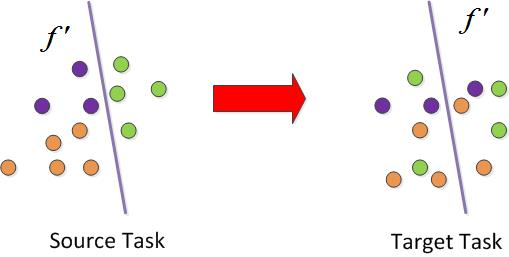
\includegraphics[scale=.5]{fig/domain2.jpg}
%\caption{Negative transfer happens when we transfer source hypothesis $f'$ to target one. Points with different color represent different categories. The data distribution would change when a new category is added into the dataset. The newly added category (red points) can also greatly affect the data distribution in target task and negative transfer could happen when we consider the multi-class scenario. }\label{fig:distribution}
\caption{Negative transfer happens when we transfer source hypothesis $f'$ to target one. Points with different color represent different categories. The data distribution would change in different domains and negative transfer could happen when we consider the multi-class scenario. }\label{fig:distribution}
\end{figure}

How to safely utilize the hypotheses to avoid negative transfer is still an open question in transfer learning \cite{Lu201514}. To avoid negative transfer, we have to evaluate the utilities of the hypothesis to keep useful knowledge and reject bad information. This approach can be achieved by setting different weights (called transfer parameters) to each hypothesis.
Previous works of HTL use Leave-One-Out error to estimate the transfer parameters and avoid negative transfer \cite{tommasi2014learning} \cite{kuzborskij2013n}. However, they try to solving a convex
optimization problem which minimizes an upper bound of
the leave-one-out error on the training set with a fix regularization term \footnote{In their original papers, this value is fixed to be 1. In our experiments, we found that this setting leads to degraded performance.}. As a result, when source and target domains are not related, previous methods suffer from negative transfer if this regularization term is not set properly (see experiments in Section \ref{sec:exp}).
In this paper, we propose our method, {called Safe Multiclass Transfer Learning (SMTLe)}, that can both alleviate negative transfer and leverage correct hypotheses to improve the performance of the target model. 
The main contributions of this paper include: (1) We propose a novel algorithm SMTLe within the HTL framework that can safely utilize the hypotheses to prevent negative transfer. We use a novel objective function with a L2 regularization term that can better estimate the transfer parameters and alleviate negative transfer. (2) We also show that by using sub-gradient descent, we can obtain the optimal solution at the rate of $O(\frac{\log(t)}{t})$ where $t$ is training iteration.
 
Our framework consists of two major phrase. In Phrase I, inspired by the previous method, we reformulate the previous HTL problem as a feature augmentation approach which reconstructs the target data by adding auxiliary features using the outputs of the source hypotheses. We show that with proper values for the transfer parameter, the target model can get improved performance by exploiting the knowledge from the source model and alleviate negative transfer.
%We also show that it is necessary to add the regularization for the transfer parameter to get improved performance of the target model.
In Phrase II, 
based on the closed-form leave-one-out (LOO) error for model evaluation, we propose our novel objective function that can better estimate the transfer parameter and alleviate negative transfer with the L2 regularization term. We prove that transfer parameters learned from our novel objection function can alleviate negative transfer. Moreover, we show that we can always find a $\frac{\log(t)}{t}$ optimal solution with $t$ iterations using sub-gradient descent while previous methods are not able to get any guaranteed convergence rate, which is a main reason why they suffer from from negative transfer.

In our experiment, initially, the data of the source and target domains are drawn from the same distribution (dataset). By adding the different level of the noise to the source data, we can generate several sources with different relatedness of the target domain. Experiment results show that when the source and target domain are related (no noise or very little noise is added), all the transfer methods can get improved result and our method outperforms the other baselines. As the source and target domain become less related, the baseline methods suffer from negative transfer while our method can still exploit knowledge from the source domain and the target model can get improved performance. 

The rest of this paper is organized as follow. In Section \ref{sec:work} we introduce the issues in transfer learning and some related work regarding these issues.
In Section \ref{sec:prob}, we reformulate the HTL in Phrase I and propose our perspective of feature augmentation. We show that we can better analysis the performance of the transfer learning algorithm with feature augmentation. Then, we propose a novel objective function for transfer parameter estimation, called SMTLe in Section \ref{sec:smitle}. We show that the estimated transfer parameter can evaluate the utility of the source hypothesis and alleviate negative transfer autonomously. In Section \ref{sec:exp}, we show the performance comparison between SMTLe and other baselines on a variety of experiments on MNIST and USPS datasets.
